\documentclass[11pt,reqno]{beamer}
\usepackage[utf8]{inputenc}
\usepackage[LGR,T1]{fontenc}
\usetheme{Dresden}
\usecolortheme{beaver}
\usepackage{amsmath}
\usepackage{amsthm}
\usepackage{amsfonts}
\usepackage{graphicx}
\usepackage{animate}
\usepackage{media9}
\usepackage[absolute,overlay]{textpos}
\usepackage{calc}
\usepackage{xcolor}
\usepackage{tcolorbox}
\usepackage[autocite=superscript, backend=biber, natbib=true]{biblatex}
\usepackage{appendixnumberbeamer}

\newcommand{\textgreek}[1]{\begingroup\fontencoding{LGR}\selectfont#1\endgroup}
\newcommand{\D}[2]{\frac{\mathrm{d} #1}{\mathrm{d} #2}}
\newcommand{\e}{\mathrm{e}}
\newcommand{\I}{\mathrm{i}}

\newcommand{\DD}[2]{\frac{\mathrm{d}^2 #1}{\mathrm{d} #2^2}}
\newcommand{\bigO}[1]{\text{O}\left(#1\right)}
\renewcommand{\P}[2]{\frac{\partial #1}{\partial #2}}
\renewcommand{\Re}{\operatorname{Re}}
\renewcommand{\Im}{\operatorname{Im}}
\newcommand{\EX}{\mathbb{E}}
\newcommand{\df}[1]{\mspace{2mu}  \mathrm{d}#1}
\newcommand{\reals}{\mathbb{R}}
\newcommand{\complex}{\mathbb{C}}
\newcommand{\conj}[1]{\overline{#1}}
\definecolor{lred}{rgb}{1,0.8,0.8}
\newcommand{\highlight}[1]{\colorbox{lred}{$\displaystyle #1$}}
\newcommand{\iip}[2]{\langle #1,#2\rangle}
\newcommand{\ip}[2]{\left\langle #1,#2\right\rangle}

\newcommand{\includemovie}[3]{%
	\includemedia[%
	width=#1,height=#2,%
	activate=pagevisible,%
	deactivate=pageclose,%
	addresource=#3,%
	flashvars={%
		src=#3 % same path as in addresource!
		&autoPlay=true % default: false; if =true, automatically starts playback after activation (see option ‘activation)’
		&loop=true % if loop=true, media is played in a loop
		&controlBarAutoHideTimeout=0 %  time span before auto-hide
	}%
	]{}{StrobeMediaPlayback.swf}%
}
\DeclareCiteCommand{\cite}
{\usebibmacro{prenote}}%
{%  
	\ifciteseen{}{%
		\usebibmacro{citeindex}%
		\let\thefootnote\relax%
		\footnotetext{%
			\mkbibbrackets{\usebibmacro{cite}}%
			\setunit{\addnbspace}
			\printnames{labelname}%
			\setunit{\labelnamepunct}
			\printfield[citetitle]{title}%
			\newunit%
			\printfield[]{year}%
		}%
		\let\thefootnote\svthefootnote%
	}%
	\autocite{\thefield{entrykey}}%
}
{\addsemicolon\space}
{\usebibmacro{postnote}}
%\renewbibmacro*{cite}{%
%	\iffieldundef{shorthand}
%	{\ifthenelse{\ifnameundef{labelname}\OR\iffieldundef{labelyear}}
%		{\usebibmacro{cite:label}%
%			\setunit{\addspace}}
%		{\printnames{labelname}%
%			\setunit{\nameyeardelim}}%
%		\usebibmacro{cite:labelyear+extrayear}%
%		\setunit{\addcomma\space}%
%		\usebibmacro{journal}}
%	{\usebibmacro{cite:shorthand}}}
\graphicspath{{./},{../images/}}
\addmediapath{{./anims/},{.}}
\title{Synchronisation}
\author{Peter Cudmore}
\bibliography{references}
\setbeamertemplate{navigation symbols}{} 

\begin{document}
\begin{frame}
	\titlepage
	\addtocounter{framenumber}{-1} 
\end{frame}


%\begin{frame}
%\centering
%\begin{figure}
%Synch of 64 Metronomes; Ikeguchi Laberatory.
%https://www.youtube.com/watch?v=4ti3d3ls5Zg
%\end{figure}
%\end{frame}
\section{Introduction}
\subsection{Motivation}
\begin{frame}{What is synchronisation?}
Synchronous\cite{synch}\\

\vspace{5pt}
From: Greek \textgreek{qr'onos} (\emph{chronos}, meaning time) and \textgreek{s'un} (syn, meaning \emph{same})\\
\vspace{5pt}

Translated: 'Sharing the common time' or 'sharing the same time'
\end{frame}

\begin{frame}{Example: Fireflies\cite{Yiu2017}}
\begin{figure}
\animategraphics[autoplay, loop, width=0.7\linewidth]{3}{anims/fireflies-}{0}{25}
\caption{\emph{Photonius carolinus} in Elkmont, Tennessee}
\end{figure}
\end{frame}
\begin{frame}{Example: Neuronal Systems\cite{Buzsaki:2004aa}}
\begin{figure}
\includegraphics[height=0.3\textheight]{science_2004_f1}
\caption{Power spectrum of hippocampal EEG in the mouse during sleep and waking periods.}
\end{figure}
\end{frame}
\begin{frame}{Example: Coupled Genetic Clocks\cite{Danino:2010aa}}
%\includemovie{.85\textheight}{.85\textheight}{movies/nature08753-s2.mov}
\begin{figure}
\includegraphics[width=0.95\linewidth]{nature08753-f12}
\end{figure}
\end{frame}
\begin{frame}{A Definition}

\begin{tcolorbox}[notitle, boxrule=0pt, colback=lred]
\centering
	Synchronisation is the process by which weakly\\ interacting oscillatory systems adjust their behaviour\\ to form a collective rhythm.
\end{tcolorbox}
	\begin{columns}
		\scriptsize
	\begin{column}{0.49\textwidth}
		\begin{figure}
			\includegraphics[scale=0.70]{synch1.pdf}
			\caption{Unsynchronised motion: oscillators rotate at different angular velocities.}
		\end{figure}
	\end{column}
	\begin{column}{0.49\textwidth}
		\begin{figure}
			\includegraphics[scale=0.70]{synch2.pdf}
			\caption{Synchronised motion: all oscillators rotate at the same angular velocity.}
		\end{figure}
	\end{column}
\end{columns}
\end{frame}
\begin{frame}{More Examples from biology}
Other examples of biological phenomenon with experimental evidence of synchronisation include\cite{synch}:
\begin{itemize}
	\item Circadian oscillations in cells,
	\item Entrainment of cardiac rhythms,
	\item Ultradian glucose-insulin oscillations in humans,
	\item Glycolytic oscillators in yeast cells,
	\item Predator-prey cycles,
	\item The cell cycle and mitosis in malignant tumors.
	\item Epileptic seizures
\end{itemize}
\end{frame}
\section{Anatomy of an oscillator}
\begin{frame}{Dynamics in the complex}
\begin{tcolorbox}[notitle, boxrule=0pt, colback=lred]
\centering
An oscillator is a dissipative autonomous\\ system with a stable periodic solution.
\end{tcolorbox}
\vfill
The key parameter of an oscillator is the natural frequency $\omega$.\\
\vfill
For a \emph{stable} $T$ periodic solution $x(t+T;x_0) = x(t;x_0)$ of the system $\dot{x} = f(x)$, the frequency and period is related by
\[
\omega = \frac{2\pi}{T}.
\]
\end{frame}
\begin{frame}{Example: Phase Oscillator}
\begin{minipage}{0.65\textwidth}
Linear Motion on $S^1$;
\[
\dot{\theta} = \omega \qquad  \theta \in [0,2\pi)
\]
is an oscillator with \emph{natural frequency} $\omega$.

The stable solution is:
\[
\theta(t) = \omega t + \theta_0 \mod 2\pi
\]
\end{minipage}
\begin{minipage}{0.3\textwidth}
	\animategraphics[autoplay, loop, width=\linewidth]{10}{anims/phaseosc-}{0}{24}
\end{minipage}
\end{frame}

\begin{frame}{Counterexample: Harmonic Motion}
Simple harmonic motion
\[
\dot{x}= -\omega y \qquad \dot{y} = \omega x
\]
 is \emph{not} an oscillator, since it is not dissipative.
\end{frame}
\begin{frame}{Example: Stuart-Landau Oscillator}
\begin{minipage}{0.65\textwidth}
Systems with a stable limit cycle are\\ oscillators and can conveniently be\\ represented by $z \in \mathbb{C}$ such that
\[
\dot{z} = \alpha(1-|z|^2)z + \I(\omega -d|z|^2)z
\]
correct to third order in $z$.
\end{minipage}
\begin{minipage}{0.3\textwidth}
	\animategraphics[autoplay, loop, width=\linewidth]{10}{anims/limitosc-}{0}{99}
\end{minipage}
\vfill

The stable periodic solution is motion on the unit circle, with frequency $\omega_\text{eff} = \omega - d$.
\end{frame}
\section{Coupled Phase Oscillators}
\begin{frame}{Heterogeneous Oscillators}
Consider $n$ phase oscillators
\[
\dot{\theta}_j = \omega_j, \qquad \theta_j \in [0,2\pi)\qquad j = 1 \ldots n.
\]
where $\omega_j$ are IID random variables with distribution $g$.
\begin{figure}
\animategraphics[autoplay, loop, height=0.6\textheight]{10}{anims/Nphaseosc-}{0}{249}
\caption{$n=25$ with Cauchy distributed $\omega_i$ and $\theta_i(0) = 0$}
\end{figure}
\end{frame}
\begin{frame}{Hetergeneous Coupled Oscillators}
Consider $n\gg1$ phase oscillators $\theta_j \in [0,2\pi)$

\[
\dot{\theta}_j = \omega_j + \sum_{k=1}^n\Gamma_{jk}(\theta_k - \theta_j) , \qquad j = 1 \ldots n.
\]
where the $j$th and $k$th oscillator are coupled by some function $\Gamma_{jk}$.
\vfill
\only<2>{
It is common to take 
\[
\Gamma_{jk}(\theta_k- \theta_j) = \frac{1}{n}A_{jk}\sin(\theta_k - \theta_j + \phi_{jk})
\]
where $A_{jk}$ is the weighted adjacency matrix of the network topology and $\phi_{jk}$ is the phase lag.
}
\end{frame}

\begin{frame}{Networked Phase Oscillators}
\[
\dot{\theta}_j = \omega_j + \frac{1}{n}\sum_kA_{jk}\sin(\theta_k - \theta_j + \phi_{jk}) , \qquad j = 1 \ldots n.
\]

\begin{itemize}
	\item Interesting dynamics even for $\omega_j = \omega$ (Chimera states).
	\item Wide variety of dynamics even for $A_{jk}= K$, $\phi_{jk}$=0 (Kuramoto Model).
\end{itemize}
There is active research into
\begin{itemize}
	\item different coupling mechanisms,
    \item different network topologies,
	\item applications, particularly in neuroscience, but also other areas of biology, engineering and physics.
\end{itemize}
\end{frame}

\begin{frame}{The Kuramoto Model}
In the `complete graph' case (all-to-all coupling) $A_{jk}=K$
\[
\dot{\theta}_j = \omega_j + \frac{K}{n}\sum_k\sin(\theta_k - \theta_j) , \qquad j = 1 \ldots n.
\]

Kuramoto\cite{Strogatz00} introduced the centroid\\

\begin{minipage}{0.55\linewidth}
	$z = r\e^{\I\psi} = \frac{1}{n}\sum_k \e^{\I\theta_k}.$
	\begin{itemize}
	\item $\psi$ is the average phase,
	\item $r$ is the `order parameter' 
\end{itemize}
\end{minipage}
\begin{minipage}{0.35\linewidth}
\begin{figure}
	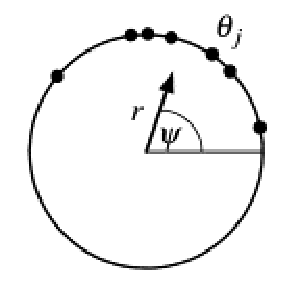
\includegraphics[height=0.35\textheight]{orderparam}
\end{figure}
\end{minipage}
\end{frame}
\begin{frame}{The Kuramoto Model II}
\[
\dot{\theta}_j = \omega_j + rK\sin(\psi - \theta_j), \qquad j = 1\ldots n
\]
\only<1>{
The Kuramoto model is arrived at by noticing that 
\[r\e^{\I\psi} = \frac{1}{n}\sum_k \e^{\I\theta_k} \implies r\e^{\I(\psi-\theta_j)} = \frac{1}{n}\sum_k \e^{\I(\theta_k-\theta_j)}
\] and equating imaginary components
\[
r\sin(\psi-\theta_j) = \frac{1}{n}\sum_k \sin(\theta_k-\theta_j)
\] 
which can be substituted into 
$
\dot{\theta}_j = \omega_j + \frac{K}{n}\sum_k\sin(\theta_k - \theta_j)$ to give the desired result.
}
\only<2>{
Some observations
\begin{itemize}
	\item All oscillators are coupled to the average phase.
	\item The strength of coupling increases as $r$ increases.
	\item If $r=1$ system is \emph{fully synchronised}; all phases are the same!!
	\item There must be a critical value for $K=K_c$ where this starts.
	\item If there is no coherent motion, oscillators are (on average) uniformly distributed between $(-\pi, \pi]$; In this situation $r\approx 0$.
\end{itemize}}
\only<3>{
Some known results\cite{Strogatz00}:
\begin{itemize}
	\item The critical coupling $K_c$ depends on the distribution $g(\omega)$. For symmetric $g$;the critical value is $K_c= 2[\pi g(0)]^{-1}$
	\item For $K > K_c$, $r$ increases to it's limiting value $r_\infty$ which also depends on $K_c$.
	\item $K < K_c$ is complicated!
\end{itemize}
}
\end{frame}

%\begin{frame}{Heterogeneous Oscillators in the Complex Plane}
%\begin{minipage}{0.5\textwidth}
%\[
%\dot{\theta}_j = \omega_j, \qquad \theta_j \in [0,2\pi)\qquad i = 1 \ldots n.
%\]
%where $\omega_j$ are IID random variables with distribution $g$.
%
%\vfill
%
%Associate each $\theta_i$ with a point in the complex plane via:
%\[
%z_j(t) = \exp(\I \theta_j)
%\]
%\end{minipage}
%\begin{minipage}{0.45\textwidth}
%\begin{figure}
%	\animategraphics[autoplay, loop, width=0.8\linewidth]{3}{anims/Ncircosc-}{0}{249}
%\end{figure}
%\end{minipage}
%
%
%\end{frame}
%
%\section{Phase Oscillators}
%\subsection{Kuramoto Model}
%\subsection{Current Areas of Research}
%
%\section{Planar Oscillators}
%\subsection{Quenching or Amplitude Death}
%\subsection{Nonlinear Coupling}

%\begin{frame}
%\tiny
%
%\printbibliography
%
%\end{frame}
\end{document}